%%%%%%%%%%%%%%%%%%%%%%%%%%%%%%%%%%%%%%%%%
% Short Sectioned Assignment
% LaTeX Template
% Version 1.0 (5/5/12)
%
% This template has been downloaded from:
% http://www.LaTeXTemplates.com
%
% Original author:
% Frits Wenneker (http://www.howtotex.com)
%
% License:
% CC BY-NC-SA 3.0 (http://creativecommons.org/licenses/by-nc-sa/3.0/)
%
%%%%%%%%%%%%%%%%%%%%%%%%%%%%%%%%%%%%%%%%%

%----------------------------------------------------------------------------------------
%	PACKAGES AND OTHER DOCUMENT CONFIGURATIONS
%----------------------------------------------------------------------------------------

\documentclass[paper=a4, fontsize=11pt]{scrartcl} % A4 paper and 11pt font size

\usepackage[T1]{fontenc} % Use 8-bit encoding that has 256 glyphs
%\usepackage{fourier} % Use the Adobe Utopia font for the document - comment this line to return to the LaTeX default
\usepackage[english]{babel} % English language/hyphenation
\usepackage{amsmath,amsfonts,amsthm} % Math packages
\usepackage[utf8]{inputenc}
\usepackage{graphicx}
\usepackage{float}
\usepackage{placeins}
\usepackage[margin=0.8in]{geometry}
\usepackage{mathtools}
\usepackage[]{algorithm2e}
\usepackage{hyperref}
\usepackage{setspace}
\usepackage{booktabs}
\usepackage[table]{xcolor}
\usepackage[T1]{fontenc}
\usepackage[utf8]{inputenc}
\usepackage{tabularx,ragged2e,booktabs,caption}
\usepackage{wrapfig}
\usepackage{array}

\usepackage{caption}
\usepackage{subcaption}
%\usepackage[style=verbose-trad2,natbib=true]{biblatex}
%\usepackage{natbib}
%\usepackage[round, comma, sort&compress]{natbib}
\usepackage{lipsum} % Used for inserting dummy 'Lorem ipsum' text into the template

\usepackage{sectsty} % Allows customizing section commands
\allsectionsfont{\centering \normalfont\scshape} % Make all sections centered, the default font and small caps

\usepackage{fancyhdr} % Custom headers and footers
\usepackage{framed}

\usepackage{listings} % Required for inserting code snippets
%\usepackage[usenames,dvipsnames]{color} % Required for specifying custom colors and referring to colors by name

\definecolor{DarkGreen}{rgb}{0.0,0.4,0.0} % Comment color
\definecolor{highlight}{RGB}{255,255,255} % Code highlight color

\lstdefinestyle{Style1}{ % Define a style for your code snippet, multiple definitions can be made if, for example, you wish to insert multiple code snippets using different programming languages into one document
language=Python, % Detects keywords, comments, strings, functions, etc for the language specified
backgroundcolor=\color{highlight}, % Set the background color for the snippet - useful for highlighting
basicstyle=\footnotesize\ttfamily, % The default font size and style of the code
breakatwhitespace=false, % If true, only allows line breaks at white space
breaklines=true, % Automatic line breaking (prevents code from protruding outside the box)
captionpos=t, % Sets the caption position: b for bottom; t for top
commentstyle=\usefont{T1}{pcr}{m}{sl}\color{DarkGreen}, % Style of comments within the code - dark green courier font
deletekeywords={}, % If you want to delete any keywords from the current language separate them by commas
%escapeinside={\%}, % This allows you to escape to LaTeX using the character in the bracket
firstnumber=1, % Line numbers begin at line 1
frame=single, % Frame around the code box, value can be: none, leftline, topline, bottomline, lines, single, shadowbox
frameround=tttt, % Rounds the corners of the frame for the top left, top right, bottom left and bottom right positions
keywordstyle=\color{Blue}\bf, % Functions are bold and blue
morekeywords={}, % Add any functions no included by default here separated by commas
numbers=left, % Location of line numbers, can take the values of: none, left, right
numbersep=10pt, % Distance of line numbers from the code box
numberstyle=\tiny\color{Gray}, % Style used for line numbers
rulecolor=\color{black}, % Frame border color
showstringspaces=false, % Don't put marks in string spaces
showtabs=false, % Display tabs in the code as lines
stepnumber=5, % The step distance between line numbers, i.e. how often will lines be numbered
stringstyle=\color{Purple}, % Strings are purple
tabsize=2, % Number of spaces per tab in the code
}

% Create a command to cleanly insert a snippet with the style above anywhere in the document
\newcommand{\insertcode}[2]{\begin{itemize}\item[]\lstinputlisting[caption=#2,label=#1,style=Style1]{#1}\end{itemize}} % The first argument is the script location/filename and the second is a caption for the listing

% Image boxes
\newcommand{\subf}[2]{%
  {\small\begin{tabular}[t]{@{}c@{}}
  #1\\#2
  \end{tabular}}%
}


\pagestyle{fancyplain} % Makes all pages in the document conform to the custom headers and footers
\fancyhead[L]{Lars Hertel} % No page header - if you want one, create it in the same way as the footers below
\fancyhead[R]{Data Analysis Report}
\fancyfoot[L]{DCARB Analysis} % Empty left footer
\fancyfoot[C]{} % Empty center footer
\fancyfoot[R]{\thepage} % Page numbering for right footer
\renewcommand{\headrulewidth}{1pt} % Remove header underlines
\renewcommand{\footrulewidth}{0pt} % Remove footer underlines
\setlength{\headheight}{13.6pt} % Customize the height of the header

\numberwithin{equation}{section} % Number equations within sections (i.e. 1.1, 1.2, 2.1, 2.2 instead of 1, 2, 3, 4)
\numberwithin{figure}{section} % Number figures within sections (i.e. 1.1, 1.2, 2.1, 2.2 instead of 1, 2, 3, 4)
\numberwithin{table}{section} % Number tables within sections (i.e. 1.1, 1.2, 2.1, 2.2 instead of 1, 2, 3, 4)

\setlength\parindent{0pt} % Removes all indentation from paragraphs - comment this line for an assignment with lots of text

%----------------------------------------------------------------------------------------
%	TITLE SECTION
%----------------------------------------------------------------------------------------

\newcommand{\horrule}[1]{\rule{\linewidth}{#1}} % Create horizontal rule command with 1 argument of height

\title{	
\normalfont \normalsize 
\textsc{University of California, Irvine} \\ [25pt] % Your university, school and/or department name(s)
\horrule{0.5pt} \\[0.4cm] % Thin top horizontal rule
\huge Quantifying the effect of DCARB on colon polyp development\\ % The assignment title
\horrule{2pt} \\[0.5cm] % Thick bottom horizontal rule
}

\author{Lars Hertel,
	ID: 61885853\\} % Your name


\date{\normalsize\today} % Today's date or a custom date

\begin{document}

\maketitle % Print the title

\begin{abstract}
In this study we aimed to quantify the effect of D-Carb on colon polyp development. We further investigated how D-Carb interacts with aspirin use and its effects on hearing over the course of approximately three years. To this end, we used data from a multi-site randomized double-blind clinical trial with 364 subjects. Treatment groups were stratified by aspirin use and a subset of 184 participants was chose to take three hearing tests over the study. We used Poisson regression to model polyp development and a linear mixed effects model to model hearing loss over time. The association between D-Carb and colon polyp development was estimated to be a 91.4\% decrease in incidence rate (95\% CI: (76.9\%, 96.8\%), p-value$<$0.001). This effect was statistically significant. Allowing for interaction with aspirin, the incidence rate among individuals on D-Carb not using aspirin was estimated to be 85.2\% (95\% CI: (55.1\%, 95.1\%), p-value=<0.001) lower than baseline (neither drug). Among individuals assigned D-Carb and using aspirin the incidence rate was 97\% lower than baseline (95\% CI: (78.1\%, 99.6\%). The interaction effect was not statistically significant (Wald test p-value=0.070). The effect of D-Carb on the average hearing threshold was estimated to be an increase of 0.769 dB (95\% CI: (0.491 dB, 1.046 dB)) over 300 days. For individuals not on D-Carb this was estimated as 0.767 dB (95\% CI: (0.498 dB, 1.035 dB)). The effect of D-Carb on hearing loss was not statistically significant.
\end{abstract}

\section{Introduction}
This study is concerned with the effectiveness of D-CARB in reducing colectoral polyp development, its effect in combination with aspirin and its potential impact on hearing loss. Colectoral cancer is the second most prevalent form of cancer in the US. One general form of colectoral cancer prevention is the monitoring and potential removal of adenomas. These colon polyps are benign tumors that can develop in the colon and have a risk of becoming malignant. An issue with this prevention approach is that large proportions of the population at risk do not undergo regular screening. As such it is of interest to inhibit the growth of adenomas. Research has found association of diet and inflammation with the development of colon polyps. However, clinical trials on dietary supplements and anti-inflammatory medication have not yielded satisfactory success. It has been found that combination chemoprevention strategies are more promising with respect to efficacy to side-effects balance. Within the realm of this report our primary goal is to assess the efficacy of D-CARB (I). This enzyme-activated inhibitor of ornithine has been shown to inhibit the start of colectoral cancer in animals. Specifically the combination with anti-inflammatory agents was shown to be successful. Other studies suggest the interaction of the two based on in vitro experimentation. Our secondary objective is thus to quantify the degree to which D-CARB interacts with non-steroidal anti-inflammatory drugs (II). As a third part of this study we want to evaluate the amount to which D-CARB has an impact on hearing loss (III). The hypothesis of this side effect arises from mouse studies where D-CARB has been shown to negatively impact hearing.

\section{Methods}
\subsection{(a)}
\label{sec:methods_a}
% Describing Sample
We base our analysis on data from a multi-site double-blind randomized clinical trial designed to assess the effects of D-CARB. The trial was conducted over the course of 36 months. The sample consists of 364 high risk patients that were consented for the study. High risk is here defined as an individual with a history of resected adenomas of 3 mm size or larger. The patients were randomly assigned in a 1:1 scheme to either treatment (600mg D-CARB once daily) or a matched placebo. The randomization was stratified on the usage of aspirin. This was in order to quantify the effect of treatment interacting with the usage of non-steroidal anti-inflammatory drugs. Here aspirin use is defined as 81 mg daily or 325 mg twice weekly. We can assume that subjects not specified as aspirin users do not use any other anti-inflammatory drugs. The aspirin use of the patient was not assigned. However, through the stratification it was ensured that each treatment arm had an equal percentage of aspirin users. Throughout the 36 months of the study participants were screened annually for adenomas.\\
In addition to this a subset of 184 participants were chosen to undergo hearing tests on an 18 month basis. All of the selected participants underwent testing at baseline and then at varying times approximately 18 and 36 months later. During the tests the individual was tested on their hearing of sound frequencies between 250 and 8000 Hz. Specifically, the procedure is to increase the sound level in steps until the patient indicates that he or she can hear the sound. The decibel level at this point is recorded. Tests are done on both the left and right ear.\\

% Comments on Sample
Overall, we are dealing with a retrospective double-blind randomized experiment. Due to the nature of a randomized experiment it may allow us to conclude cause and effect relationships.

% Introduce variables and Missingness
Variables recorded can be summarized into demographic variables and variables concerned with the hearing tests. For each study participant a unique patient ID, the study site at which the patient was recruited, whether they had been assigned treatment or placebo, their daily aspirin usage, the patient's age at time of the randomization, the patient's race and the sum of the polyps detected throughout the trial in the patient were recorded. Aspirin use was defined as above. Ethnicity as specified by the individual was recorded in levels of American Indian or Alaskan Native, Asian or Pacific Islander, Black, German/Indian/Hispanic/Spanish, Hispanic, Spanish, White or Other.\\
For the second part of the study hearing detection in decibel was measured at 250, 500, 1000, 2000, 3000, 4000, 6000 and 8000 Hz for the left and right ear. These were recorded alongside the hearing test dates and the total number of days for which treatment or placebo was received.\\
There is missingness to be found especially in the demographic data of the patients. We will go more into detail about this in section~\ref{sec:results_a}.

% Use of variables in analysis
We define the treatment variable (D-CARB vs. placebo) as predictor of interest in this study. For our second objective we define the effect of the treatment variable together with its interaction with aspirin use as the predictor of interest. For both tasks the response variable will be the number of adenomas observed throughout the study. To achieve our third goal we consider treatment and its interaction with time as predictor of interest. As response variable we consider the arithmetic average of a subject's hearing detection decibel level across the left and right ear at one test. We require a summary statistic due to the model that is being used. Furtermore, choosing the average is justified by the fact that the absolute change in hearing loss was observed to be constant across multiple sound frequencies in other experiments. In addition to that \cite{hearing_levels} recommends a simple average as summary statistic for auditory sensitivity. For the three tasks we consider all demographic variables as potential adjustment variables.

\subsection{(b)}
\label{sec:methods_b}
\subsubsection{D-CARB effect on polyp development}
\label{sec:methods_model_i_ii}
% Describe Model for I and ii
For task I and II we consider a Poisson regression model. This is motivated by the nature of the response which is measured in counts. In particular we consider modeling the incidence rate of adenomas over 36 months. Our goal is thus to compare the incidence rate in the population that receives the treatment against the population that receives the placebo. As such the log-linear Poisson regression models the log of the incidence rate as a linear combination of predictor variables. These predictor variables are the predictor of interest and possibly other observed variables. The other variables are considered adjustment variables. These serve either to improve precision on the response (precision variables) or control for confounding effects (confounding variables). An observed count is then modeled by a Poisson distribution. Its expected value is defined as the product of the incidence rate in the population that the count comes from times the exposure period. For this part of the study we consider all subjects to have the same exposure time of 36 months. It is therefore not necessary to consider individual offsets. Instead we will interpret the rate over 36 months time.\\
% Interpretation of coefficients
Modeling the log-incidence rate as a linear combination of predictor variables we obtain coefficients for each predictor variable. We interpret the exponential of each of these coefficients as the incidence rate ratio (IRR) comparing two populations differing by one unit in the associated predictor variable and that are similar with respect to the other predictor variables. In the case that two variables are interacting we consider the IRR at the different levels of the second variable.\\

% Diagnostics
After fitting the model we assess the appropriateness of the fit. We consider a Pearson residual plot to assess the model specification. We expect the squared Pearson residuals to be constant around 1. In the case that we find this not to be true we assume that the mean-variance assumption is violated. We then consider scaling by an estimated constant overdispersion factor. However, if the variance is not observed to be constant as a function of the fitted values we will revert to the robust variance estimator as proposed in~\cite{sandwich}. The use of the robust variance estimator is justified in this study since the sample size is large enough. The specification of the functional form may be checked in a Poisson regression using Partial residuals. In this case this is not a primary concern since the predictor of interest is an indicator variable and its interaction with aspirin-use is also binary. In order to assess influential data points we will consider deviance residuals and delta beta plots. In the former we will flag points whose absolute residual is larger than the 97.5th percentile of the normal distribution. For the delta beta values we will consider removing points whose value is higher than 0.1. We will only consider delta beta diagnostics for the predictor of interest.\\

%% Model building
% Intro

% Philosophy
We specify the model a priori. That means we decide on model, adjustment variables and functional form before taking the data into account. We do this in order to achieve maximal generalizability of the results. We may however adjust standard errors if model diagnostics indicate that the standard error estimates obtained from the model fit are incorrect. We revert to a standard functional form for all predictors since a priori there is no evidence that suggests any other particular form for the predictor of interest or the adjustment variables. In general, adjustment variables are chosen as precision variables or confounding variables. In our case we are less concerned with confounding variables. This is because treatment assignment was randomized. Hence it can be assumed that the correlation of the predictor of interest with any other adjustment variable is close to zero. In the frame of this report we were not able to show whether an interaction of a randomized treatment with an observed variable may be correlated to other observed variables. It is however in our case not an issue since we will adjust for the interacting variable.\\

% Factors of Response
We consider predictors of the response variable. Here, we are thinking about what might increase the rate of adenomas in general terms since the actual count will be non-linearly related to any predictors.
% Research suggested variables
According to~\cite{mayoclinic} risk factors for the formation of colon polyps or cancer include being over 50 years of age, inflammatory intestinal conditions, family history of colon cancer, tabacco and alcohol use, obesity and lack of exercise, ethnicity (African Americans have a higher risk) and not well controlled Type 2 diabetes. \cite{kahn} reports that in an observational study of 7504 men and 5111 women, after adjustment for family history of colon cancer and age, increased odds of colon cancer were found for smoking, high alcohol consumtion and high body mass index. High exercise level and aspirin use in women was inversely associated with the odds of colon polyps. The summary of risk factors in~\cite{grahn} highlights African Americans as being at higher risk, men being at higher risk than women and confirms smoking, obesity and inflammation as risk factors.\\

% Table
\begin{wraptable}{l}{8cm}
\centering
\caption{Patient characteristics.}
\label{tab:characteristics}
\begin{tabular}{m{3cm} m{2cm} l}
  \hline
Variable & count (proportion) & NAs \\ 
  \hline
site & --- & 0 \\ 
  site: 1 & 68(18.68\%) &  \\ 
  site: 2 & 40(10.99\%) &  \\ 
  site: 3 & 57(15.66\%) &  \\ 
  site: 4 & 32(8.79\%) &  \\ 
  site: 5 & 49(13.46\%) &  \\ 
  site: 6 & 72(19.78\%) &  \\ 
  site: 8 & 9(2.47\%) &  \\ 
  site: 9 & 4(1.1\%) &  \\ 
  site: 11 & 33(9.07\%) &  \\ \hline
  tx & 182(50\%) & 0 \\ \hline
  asa\_use & 138(38\%) & 0 \\ \hline
  sex & --- & 8 \\ 
  Female & 88(24.72\%) &  \\ 
  Male & 268(75.28\%) &  \\ \hline
  ethnic & --- & 12 \\ 
  American Indian or Alaskan Native & 1(0.28\%) &  \\ 
  Asian or Pacific Islander & 13(3.69\%) &  \\ 
  Black & 14(3.98\%) &  \\ 
  German, Indian, Hispanic, Spanish & 1(0.28\%) &  \\ 
  Hispanic & 25(7.1\%) &  \\ 
  Other & 3(0.85\%) &  \\ 
  Spanish & 1(0.28\%) &  \\ 
  White & 294(83.52\%) &  \\ \hline
  adenomas & --- & 0 \\ 
  adenomas: 0 & 300(82.42\%) &  \\ 
  adenomas: 1 & 25(6.87\%) &  \\ 
  adenomas: 2 & 21(5.77\%) &  \\ 
  adenomas: 3 & 10(2.75\%) &  \\ 
  adenomas: 4 & 4(1.1\%) &  \\ 
  adenomas: 5 & 3(0.82\%) &  \\ 
  adenomas: 6 & 1(0.27\%) &  \\
    \hline
 & median (SD) & NAs \\ 
  \hline
age & 60.88(8.39) & 8 \\ 
   \hline
\end{tabular}
\end{wraptable}

% Association with predictor of interest / interaction
Due to the randomized treatment assignment we can assume that there is no correlation between treatment assignment and any of these risk factors. There may however be association between aspirin use and any of these variables. We consider that aspirin use might be positively associated with age.
% Proxies for these in our dataset
We consider which of the variables described in~\ref{sec:methods_a} might be used as proxies for the risk factors of colon cancer as found by previous research.
% age
We have a recording for age to match the increased risk of colon cancer at higher age.
% aspirin
We have a recording of aspirin use. This may be taken as a proxy of inflammation since regular aspirin use may only be prescribed if the individual has inflammation problems. 
% sex
The variables include a recording of the individual's gender which matches the higher risk factor for men.
% ethnic
Finally, we have information on the participants ethnicity or race.
% others
We do not have information on diet, tabacco and alcohol use, obesity or lack of exercise. Study site might be a predictor of diet in certain cases.\\


% Our model
We decide to include age, aspirin use, gender and race African American vs. other as adjustment variables.
There is not a clear consensus from the sources cited above whether increasing age plays a role or just being older than a threshold (for example 50 years of age) would be relevant.
Aspirin use might itself be a predictor of inflammation so it makes sense to include it. Furthermore, it should be included as a main effect in the model where it interacts with the treatment.

Gender is included due to the fact that men might be at higher risk.
Finally we include race as a factor with African American or not. This is because two of the three sources cited above stated African Americans as being at higher risk. Across other races there was no clear consensus how race is related with risk of colon cancer. From a statistical point of view we consider that only 14 African American participants were in the study. We can expect that the estimate for the coefficient of this subpopulation will be highly variable. However, this does not increase the variance on the estimate of the treatment coefficient. Furthermore, estimating only one race vs. baseline only decreases the degrees of freedom in the model by one. The overall estimates will thus not be impacted much. At best we gain precision on the predictor of interest.
We do not include study site as a predictor because we conclude that it will at best be a weak predictor of diet and be negatively impacting efficiency due to the 9 levels of this variable. We use the same adjustment variables for the interaction model in task II.\\

% Missing values
We conduct a complete case analysis. That means that we discard observations with missing values and implicitly assume that the missingness has no impact on the estimated effect of the treatment. We make this assumption since missingness only occurs in the demographic information. This was collected at the time of randomization. It is thus a fair assumption that the way demographic information is missing has no correlation with the randomization or the impact of the treatment.\\

\subsubsection{D-CARB effect on hearing loss}
\label{sec:methods_model_iii}
% Model description
In order to assess the relationship between D-CARB and hearing loss we use a linear mixed effects model. We have a continuous, positive response variable and both continuous and categorical predictor variables. We have three hearing tests for each subject at three different times. The fact that measurements within a subject are expected to be correlated violates the independence assumption of linear regression. A linear mixed effects model deals with this by allowing for different variances for observations within one subject and between subjects. Specifically, we allow for a subject specific intercept and slope. Using this model we allow observations that are further apart in time to have less correlation than observations that are close to one another.\\

\begin{wrapfigure}{r}{0.5\textwidth}
  \begin{center}
    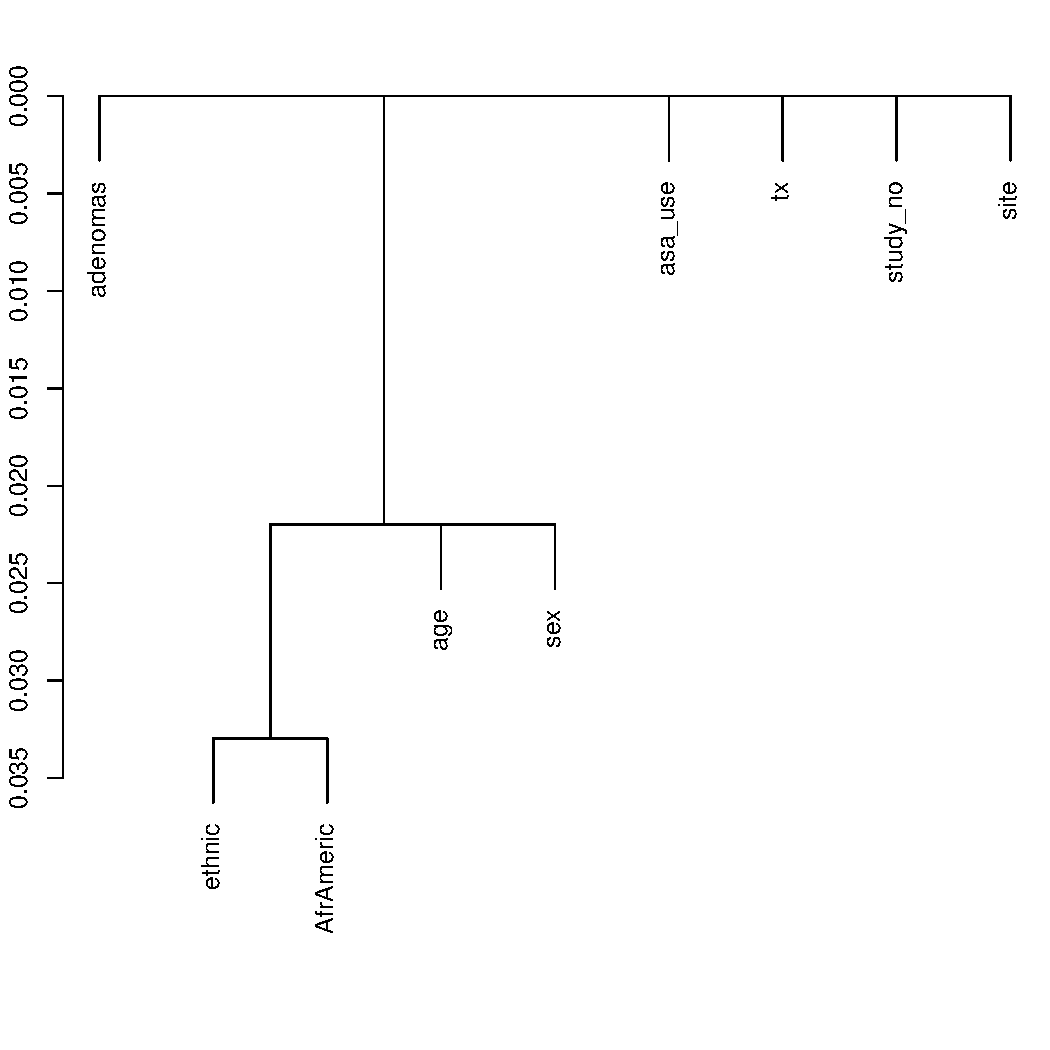
\includegraphics[width=0.38\textwidth]{./rcode/plots/na_patterns}
  \end{center}
  \caption{Missingness patterns in the demographic data of the study participants. The diagram indicates that ethnicity, age and sex tend to be missing together.}
  \label{fig:na_patterns}
\end{wrapfigure}

% Interpretation of coefficients
We are primarly interested in the estimates of the fixed effects. Each fixed effect represents a marginal estimate across all subjects. In this model fixed main effects are interpreted as the difference in the mean response between two subpopulations that differ by one unit in the respective predictor. Note that the fixed effects are concerned with the effect across subpopulations such that the indiviual level random effects have zero expectation.\\

% Diagnostics
There are multiple assumptions to be assessed when using the linear mixed effects model. Most importantly, the mean structure should be checked. We will do this using residual vs. fitted value plots. We refer to the shape of the residual vs. fitted value plot for the variance specification. Finally, to check the normality assumption of the error term we consider Normal Q-Q plots.\\

% Predictors of the response
Again we consider general predictors of the response, here hearing loss. \cite{mayohearing} lists risk factors in hearing loss as aging, short term loud noise, heredity, long term loud noises, certain antibiotics and chemotherapy drugs and certain illnesses. According an observational study analysed in~\cite{lin} age, sex and race are associated with hearing loss. They too found negative association of being African American with hearing loss. \cite{agrawal} states that after adjusting for age, sex, ethnicity and educational level, smoking and diabetes were positively associated with increased hearing thresholds.\\

% Proxies in our dataset
From the risk factors listed above we have matching variables of age, sex and ethnicity in our dataset.

% Our model
We decide that we adjust for age and sex. We do not include African American ethnicity since none of the 14 African American participants were in the hearing loss subexperiment. We condition on the treatment and let treatment interact with the time between the hearing test and the beginning of the study. We note that there is a further measurement of time on treatment. The individual may have stopped the treatment before the third hearing test for various reasons. Since the time difference between the stop of the medical treatment and the last hearing test is small in most cases and in order to keep the model simple we ignore this in our primary model.
% Missingness
Therefore, as for task I and II we do a complete case analysis for our primary model for task III. %Contrary to the demographic data used in I and II, the longitudinal audio data has missing data that may not be missing completely at random. In fact, the treatment effect could be related to missing data in the hearing tests or premature ending of the treatment. We will address these issues further in the secondary analysis.
%% CAREFUL: am I addressing these questions?

\begin{wrapfigure}{l}{0.5\textwidth}
  \begin{center}
    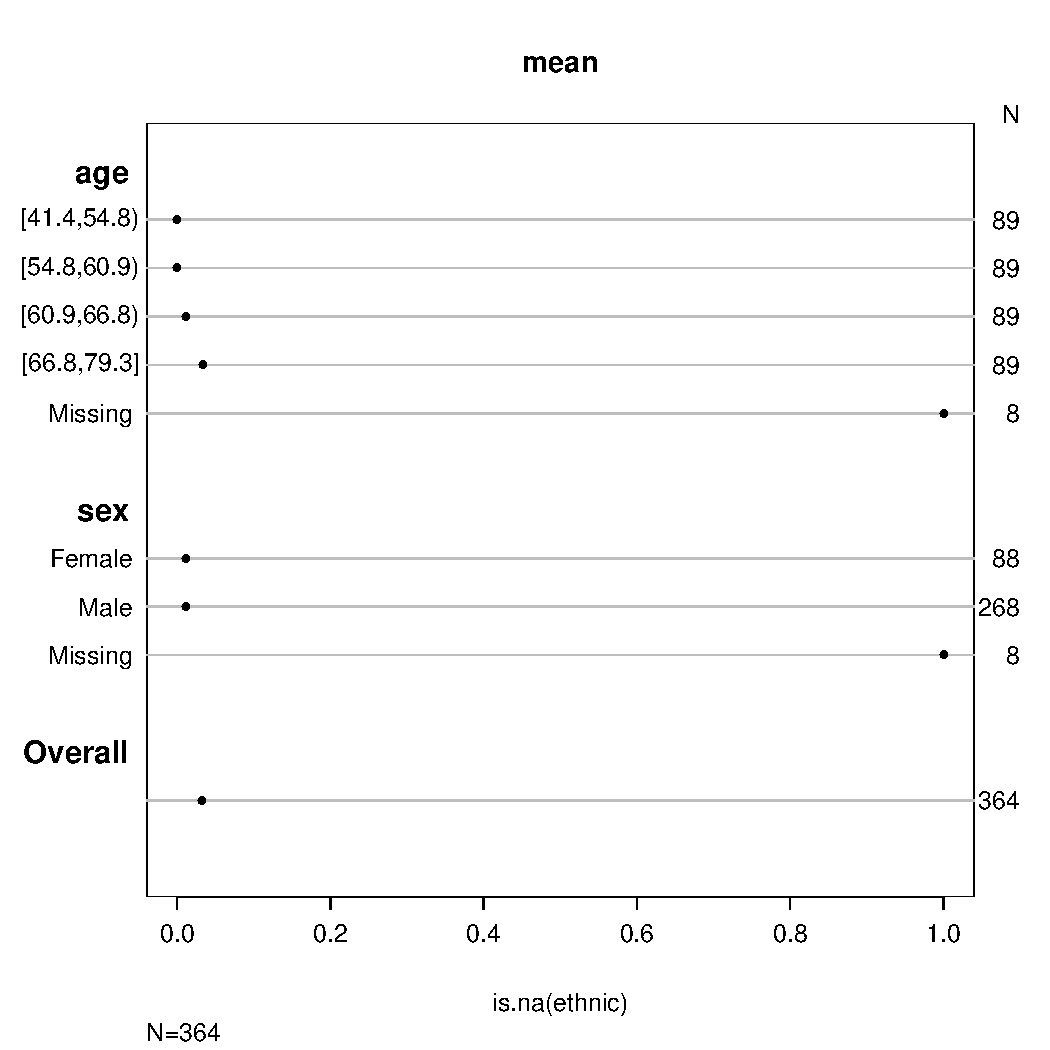
\includegraphics[width=0.38\textwidth]{./rcode/plots/na_ethnic_regressed}
  \end{center}
  \caption{Proportion of missingness of the levels of age and sex together with ethnicity. The plot shows that all individuals that are missing their gender information are also missing ethnicity information. Similarly, all individuals that are missing their age information are also missing their ethnicity status. Furthermore, some individuals in the 61 to 67 year group and in the 67 to 79 year group are also missing their ethnicity information.}
  \label{fig:na_ethnic_regressed}
\end{wrapfigure}

\section{Results}
\subsection{(a)}
\label{sec:results_a}
% EDA
We present descriptive statistics of the sample. Table~\ref{tab:characteristics} describes the sample in terms of the patient characteristics. We note that study site 8 and 9 had a very small proportion of participants. As expected exactly 50\% of participants received the treatment. There were 38\% of participants that were classified as aspirin users. These were equally divided into both treatment groups via the stratification. The proportion of males in the sample was three times higher than that of females. Eligible study participants have to be high risk participants first of all. The higher proportion of men could indicate that there are more high risk individuals that are men. There are 8 observations with missing gender status. By far the largest ethnical group in the sample were white. This could stem from whites being at higher risk of colon cancer. However, it is more likely that the study sites were in predominantly ethnically white locations or there is a higher proportion of whites that get screened for colon cancer. There are 12 missing observations of ethnicity. We consider the age variable, with mean 60.88 years and standard deviation 8.39. Furthermore, the minimum age was 41 and the highest age 79. The distribution was approximately symmetric with the median being approximately 61 years.
% histogram of age in the appendix?
Finally, the count of observed adenomas is presented with the minimum being 0 and the maximum 6. The majority of participants were not observed to have developed adenomas. The proportion decreases as the number of adenomas increases.\\
% STRATIFY by POI

% Missingness
We refered in table~\ref{tab:characteristics} to the number of missing values in each demographic variable. We consider the patterns of missingness in figure~\ref{fig:na_patterns} and figure~\ref{fig:na_ethnic_regressed}. Both diagrams indicate that the demographic variables etnicity, sex and age tend to be missing together. One possible explanation is that these subjects' demographic information was lost. Another explanation would be that these individuals refused to provide any information about themselves. In the worst case scenario the missingness may be related to our adjustment variables. However, we do not expect it to be related to the treatment variable since the assignment was randomized. Any impact on the estimate of the treatment effect is thus unlikely.\\


%\begin{figure}[H]
%  \centering
%  \begin{minipage}[b]{0.49\textwidth}
%    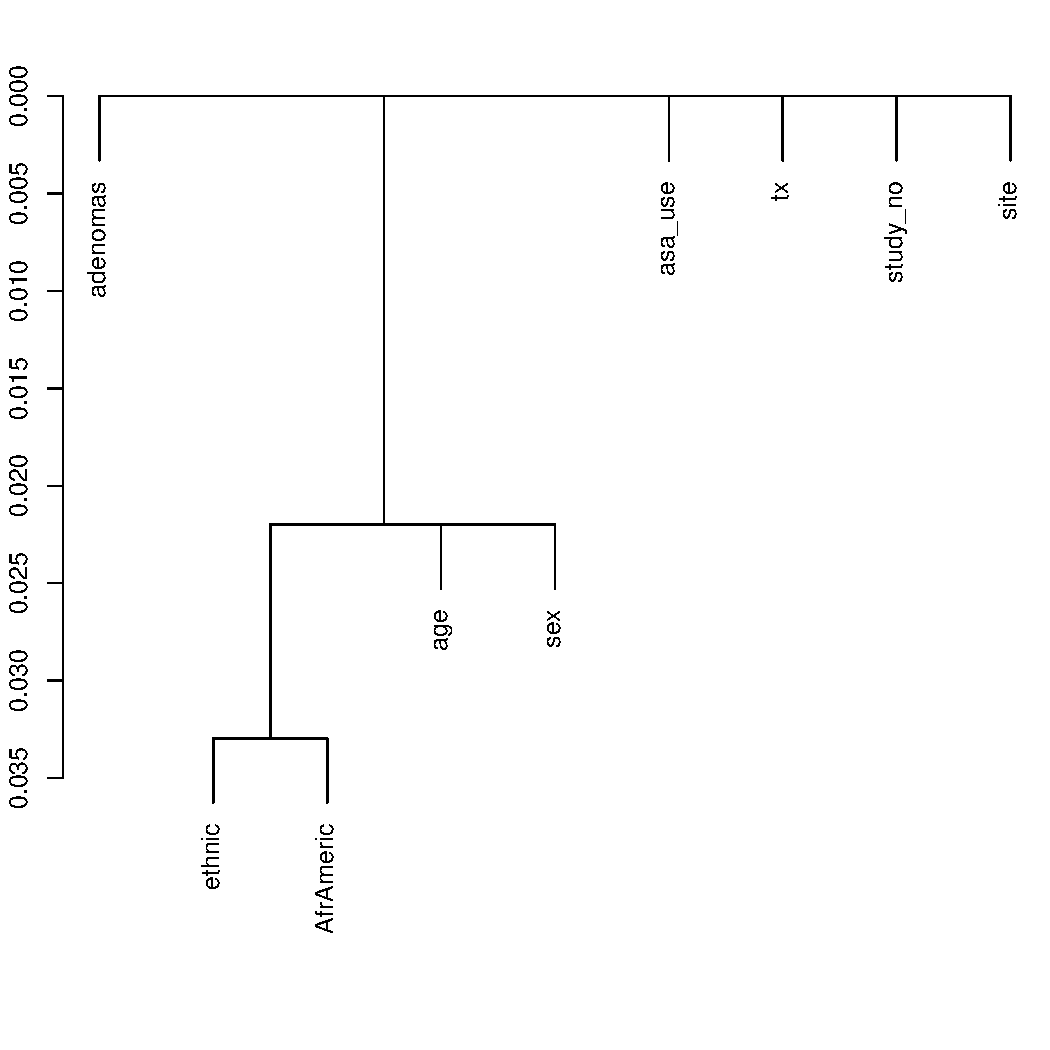
\includegraphics[width=\textwidth]{./rcode/plots/na_patterns}
%    \caption*{Missingness patterns in the demographic data of the study participants. The diagram indicates that ethnicity, age and sex tend to be missing together.}
%  \end{minipage}
%  \hfill
%  \begin{minipage}[b]{0.49\textwidth}
%    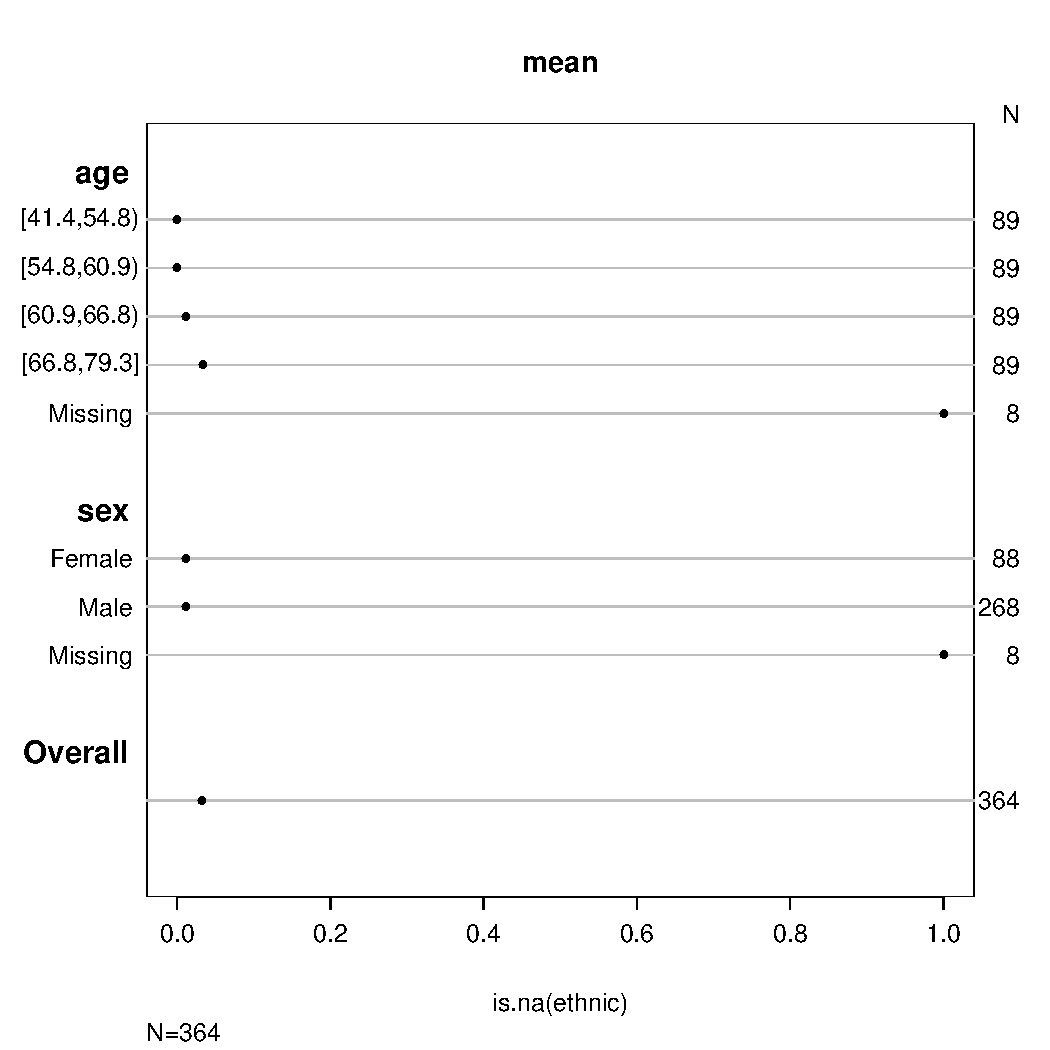
\includegraphics[width=\textwidth]{./rcode/plots/na_ethnic_regressed}
%    \caption*{Proportion of missingness of the levels of age and sex together with ethnicity. The plot shows that all individuals that are missing their gender information are also missing ethnicity information. Similarly, all individuals that are missing their age information are also missing their ethnicity status. Furthermore, some individuals in the 61 to 67 year group and in the 67 to 79 year group are also missing their ethnicity information.}
%  \end{minipage}
%\end{figure}


% Bivariate and Trivariate
Figures~\ref{fig:counts_stratified} and~\ref{fig:counts_stratified_aspirin} show counts of adenomas among treatment and placebo group. In the~\ref{fig:counts_stratified_aspirin} this is further stratified by aspirin use. The stratification by treatment group shows that the treatment group seems to have lower counts of observed adenomas overall. The sample means are $0.055$ with sample standard deviation of $0.360$ in the treatment group and $0.681$ with $1.211$ in the placebo group. Considering the stratification on aspirin use the counts show an effect of aspirin in opposite directions depending on the treatment group. Among the treatment group it seems to be associated with slightly lower counts (mean(standard deviation): no aspirin 0.080(0.446) vs. aspirin 0.014(0.120)). In the placebo group it appears that it correlates with higher counts of adenomas (mean(standard deviation): no aspirin 0.575(1.209) vs. aspirin 0.855(1.203)).

\begin{figure}[H]
  \centering
  \begin{minipage}[b]{0.38\textwidth}
    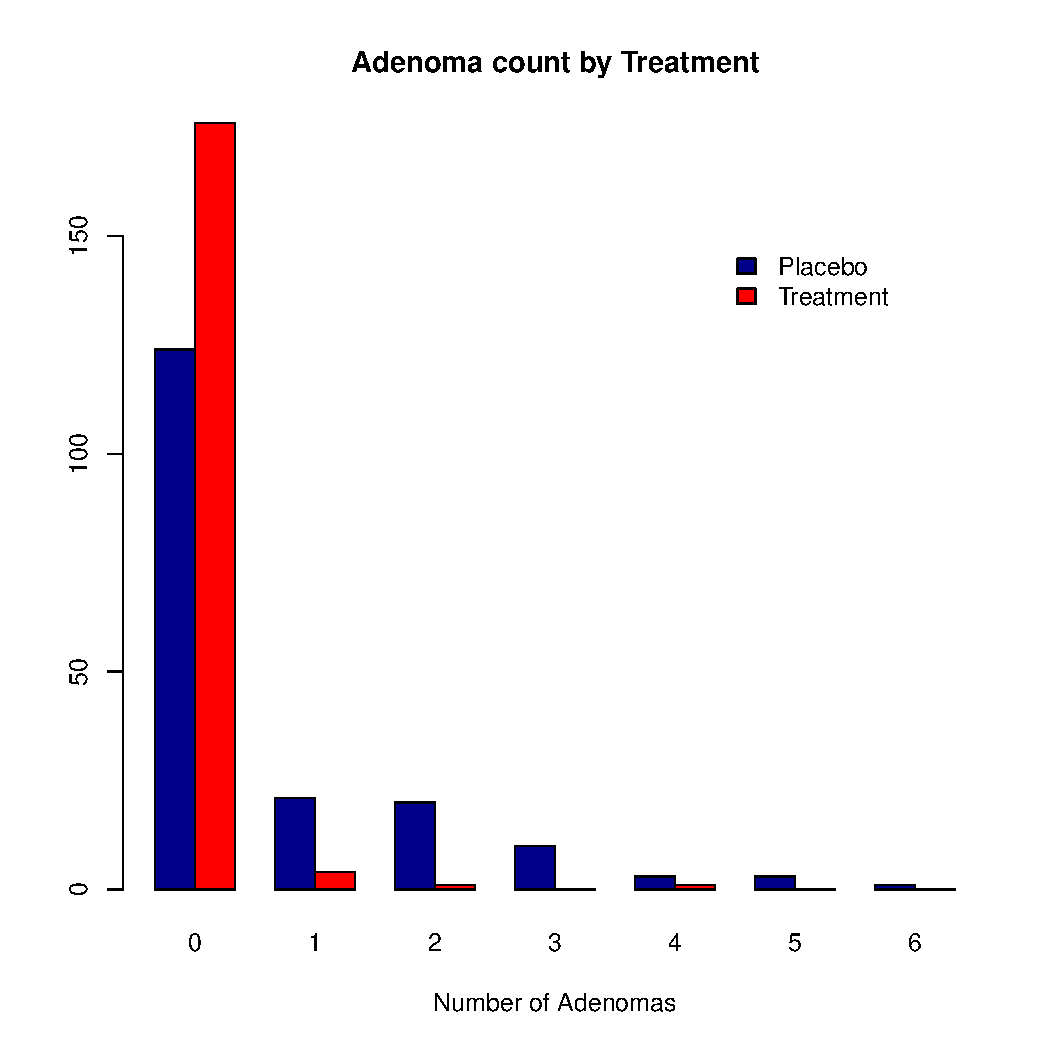
\includegraphics[width=\textwidth]{./rcode/plots/bivariate_barplot_adenomas}
    \caption{The barplot shows the counts of adenomas in the treatment (red) against the placebo (blue) group. The treatment group shows a higher number of zero counts whereas the placebo group has a higher number of counts larger than zero.}
    \label{fig:counts_stratified}
  \end{minipage}
  \hfill
  \begin{minipage}[b]{0.38\textwidth}
    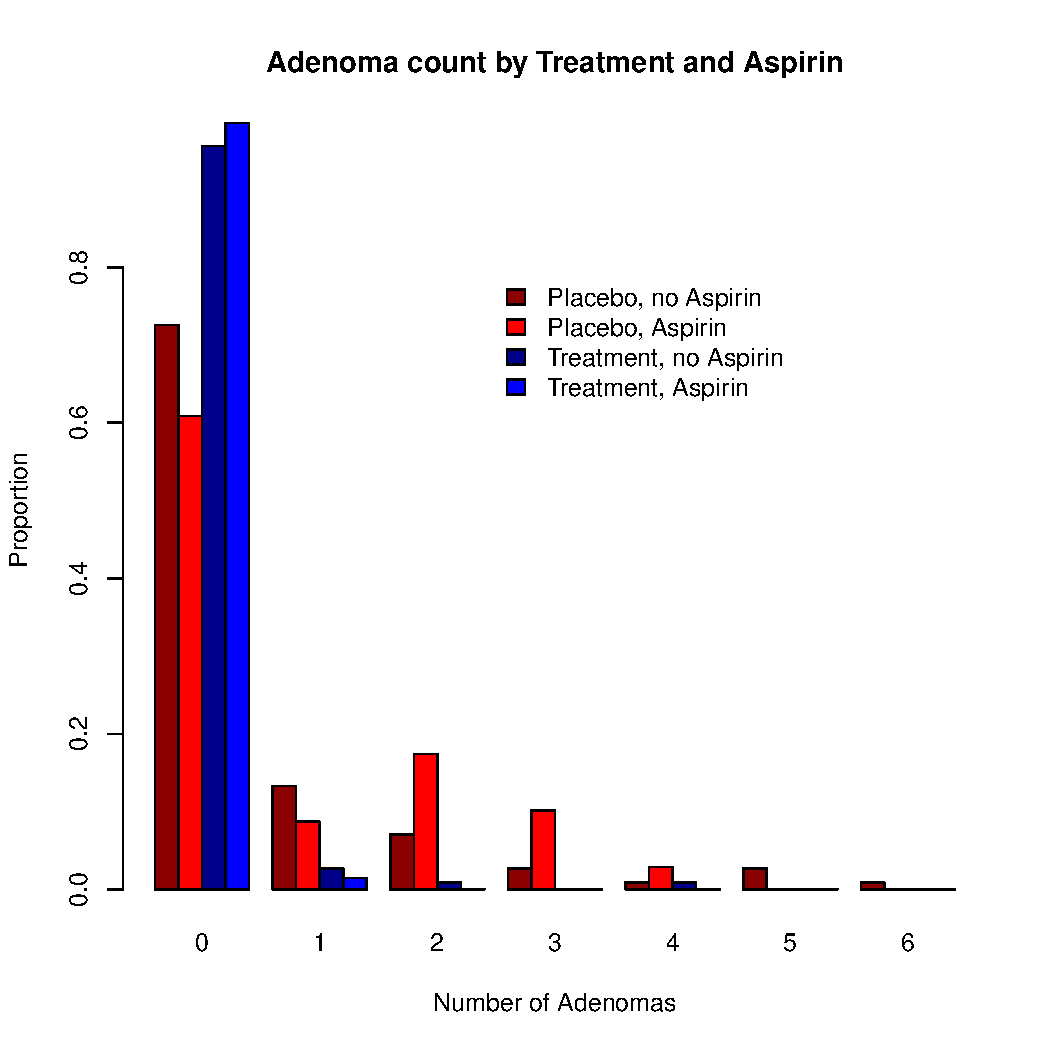
\includegraphics[width=\textwidth]{./rcode/plots/trivariate_barplot_adenomas}
    \caption{The barplot shows counts of adenomas stratified by treatment vs. placebo and aspirin use vs. not aspirin use. Among the treatment group those using aspirin had a higher count of zero adenomas and lower counts greater than zero. Among the placebo group those using aspirin had slightly lower zero and one count and much higher counts at 2 and 3.}
    \label{fig:counts_stratified_aspirin}
  \end{minipage}
\end{figure}

% Longitudinal
In order to investigate the longitudinal effects of D-CARB treatment on hearing start by considering descriptive statistics. We expect the demographics in the subsample to be similar to those in table~\ref{tab:characteristics} since a random sample was taken.
% IS THAT REALLY SO? MAKE SEPARATE TABLE FOR HEARING PEOPLE?
In figure~\ref{fig:spaghetti_plot} and~\ref{fig:time_boxplot} we show the longitudinal development of average hearing threshold against time since study start. The plot of individual line segments does not indicate a clear trend in either treatment group. The boxplot shows the distribution in each group when time since study start is grouped into three equal quantile groups. The diagram does not show an obvious trend. In the first interval the median of the treatment group is higher, in the middle interval it is lower and then in the third higher again. If the treatment group was experiencing hearing loss we would expect the median to increase with respect to time and the placebo group.\\
We also consider the time between the last treatment was taken by the participant and he or she took the last hearing test in figure~\ref{fig:days_since_last_trt}. For the majority of participants this time is under 100 days with outliers at 250 days and over a year. However, the distribution does not seem to differ significantly between treatment groups. Thus our simplification of modeling the average hearing threshold with respect to the time between study start and hearing test does not seem too strong.


\begin{figure}[H]
  \centering
  \begin{minipage}[b]{0.38\textwidth}
    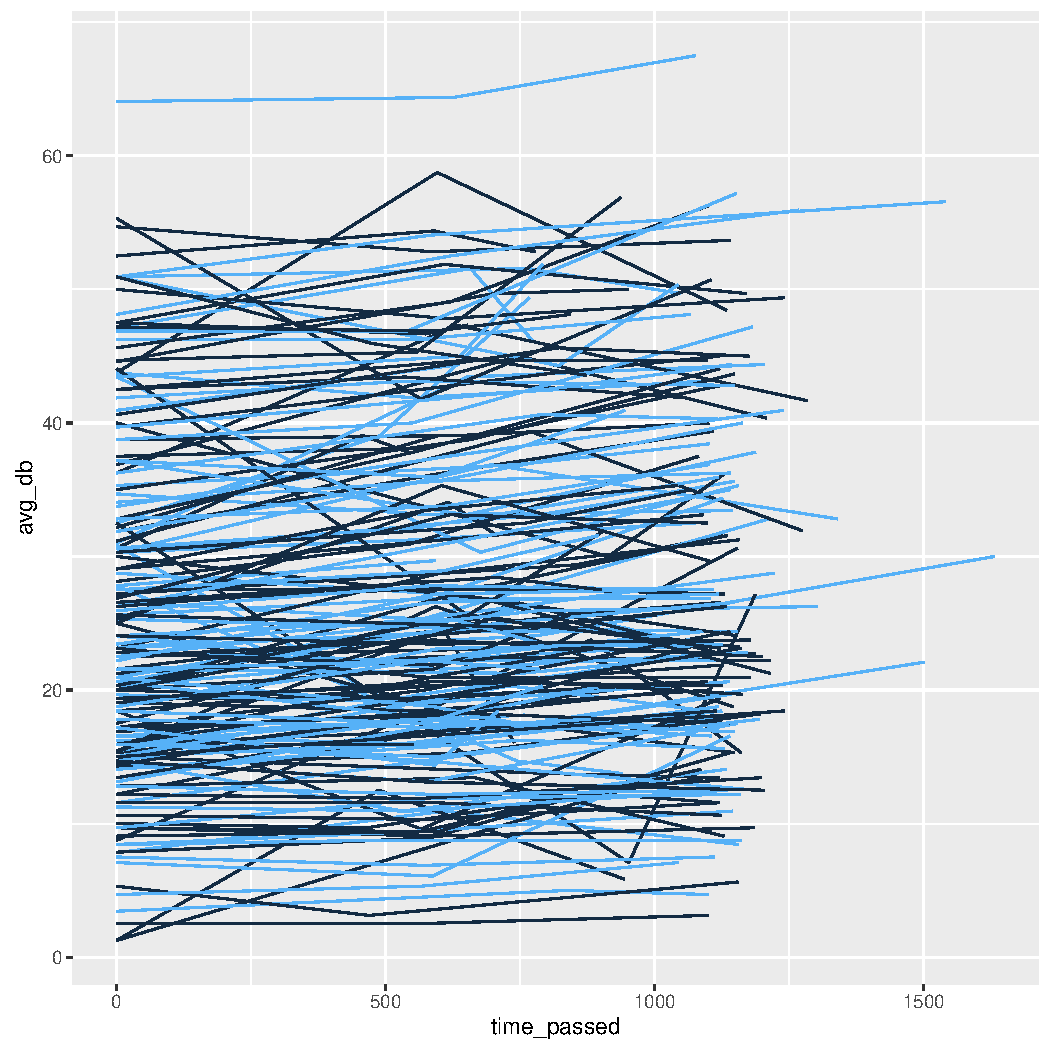
\includegraphics[width=\textwidth]{./rcode/plots/longitudinal}
    \caption{Line segments indicating the development of the participants hearing threshold over time since study start. Blue lines correspond to the treatment group, black lines to the placebo group.}
    \label{fig:spaghetti_plot}
  \end{minipage}
  \hfill
  \begin{minipage}[b]{0.38\textwidth}
    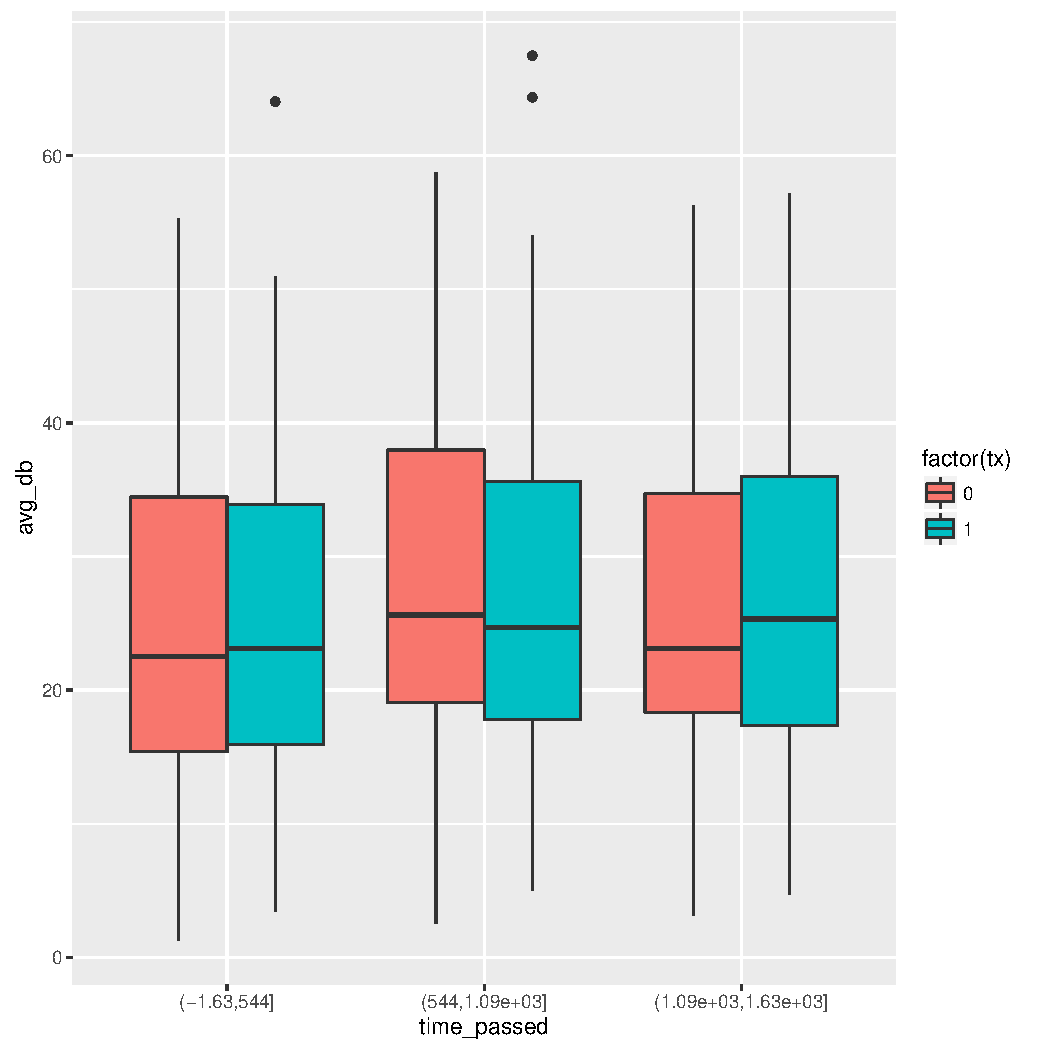
\includegraphics[width=\textwidth]{./rcode/plots/longitudinal_box}
    \caption{Boxplots with time since study start quantized into three percentile groups against average hearing threshold across measure frequencies stratified by treatment(green) vs. placebo(red).}
    \label{fig:time_boxplot}
  \end{minipage}
\end{figure}

\subsection{(B)}
\label{sec:results_b}
% Primary Analysis
In this section we present the models to quantify the effect of D-CARB treatment on colon polyp development, quantify D-CARB's interaction with aspirin and assess its potential negative effect on hearing (models I to III, respectively). We choose adjustment variables a priori as described in section~\ref{sec:methods_b}.

% Model I
Table~\ref{tab:model_i_results} shows Poisson regression estimates of the incidence rate ratio (IRR) of each variable, a 95\% confidence interval on the incidence rate ratio and the corresponding p-value. The confidence intervals and p-values are based on standard errors that have been computed using the robust variance estimator.
% Diagnostics
This was motivated by model diagnostics presented in appendix~\ref{sec:model_i_app}. The Pearson residual plot indicates that the mean-variance relationship is misspecified. Since a smoother line indicates a curved line we conclude that the standard error is not constant across the fitted values. We therefore employ the robust variance estimator rather than estimating an overdispersion coefficient. The deviance residuals (figure~\ref{fig:model_i_diagnostics} (a)) indicate multiple flagged points. We do not remove any of these due to the large number of points. We find three highly influentual points in the treatment delta-beta plot. Again we do not remove these points.
%Indeed, two of them correspond to individuals with 5 and 6 observed adenomas. The third individual is female, 
% ATTENTION: PROBLEM HERE. WHO ARE THE HIGH DF BETA INDIVIDUALS??? NEED TO BE INVESTIGATED
% Interpretation
We conclude that among high risk individuals the estimated incidence rate ratio of colon polyp development between individuals that receive D-CARB treatment and individuals that are similar with respect to aspirin use, age, sex and ethnicity and who receive a placebo is 0.086 (95\% CI: (0.032, 0.231), p-value: <0.001). We also note that the increased incidence rate among aspirin users may be due to our assumption that aspirin may be a proxy for inflammation.\\

% Model II
The second model is concerned with the effect of aspirin and D-CARB together. The question of interest is whether there is an interacting effect between aspirin and D-CARB. Table~\ref{tab:model_ii_results} shows estimates of the incidence rate ratios of polyp development for the coefficients in the model against their baseline. The confidence intervals and p-values are based on standard error estimates from the robust variance estimator. Model diagnostics are discussed in appendix~\ref{sec:model_ii_app}. Similar to model I, diagnostic plots indicate that the mean-variance specification is incorrect. In order to obtain valid inference we re-estimate standard errors. We consider outliers and influential points (figure~\ref{fig:model_ii_diagnostics}) but do not remove any observations.\\

\captionsetup{width=.5\textwidth}
\begin{wraptable}{l}{8cm}
\centering
\caption{Poisson regression estimates of the incidence rate ratios of polyp development.}
\label{tab:model_i_results}
\begin{tabular}{m{2cm} m{3.5cm} l}
  \hline
 & Incidence Rate Ratio (95\% CI) & p-value \\ 
  \hline
%Intercept & 1.562 (0.251, 9.731) & 0.633 \\ 
  no D-Carb & 1.0 & \\
  D-Carb & 0.086 (0.032, 0.231) & $<$0.001 \\ 
  no Aspirin & 1.0 &  \\ 
  Aspirin & 1.467 (0.913, 2.356) & 0.113 \\ 
  Age (yrs) & 0.983 (0.953, 1.013) & 0.256 \\ 
  Male & 1.097 (0.584, 2.061) & 0.773 \\ 
  African American & 0.653 (0.106, 4.016) & 0.645 \\ 
   \hline
\end{tabular}
\end{wraptable}

% Interpretation
From model II we estimate that the incidence rate for aspirin users that take the placebo is 65\% higher than non aspirin users (95\% CI: (1\%, 170\%), p-value=0.046). Given the fact that aspirin use might indicate inflammation which is a risk factor in colon polyp development this result is in line with our a prior assumptions. The incidence rate of individuals on D-Carb who do not use aspirin is estimated to be 85.2\% lower (95\% CI: (55.1\%, 95.1\%), p-value=<0.001) than for individuals who do not use aspirin or D-Carb. Finally, the incidence rate for individuals that use aspirin and D-Carb is estimated to be 97\% lower than for individuals from the baseline group (95\% CI: (78.1\%, 99.6\%), p-value=<0.001). We note that the interaction itself is not statistically significant when considering the Wald test (p-value=0.070). %Conducting the likelihood ratio test between model I and model II we reject model I. This means the interaction is statistically significant according to the likelihood ratio test (p-value=0.014).
We rely on the Wald statistic here because it is the easiest to compute when using the robust variance estimator. While the likelihood ratio test may be more stable, computing its test statistic is more complex in the situation of non-constant overdispersion. Furthermore, we assume that since the sample size is large enough the difference between the tests will be marginal.\\

\captionsetup{width=.5\textwidth}
\begin{wraptable}{l}{10cm}
\centering
\caption{Poisson regression estimates of the incidence rate ratios of polyp development for interactions with Aspirin use.}
\label{tab:model_ii_results}
\begin{tabular}{m{4cm} m{3.5cm} l}
  \hline
 & Incidence Rate Ratio (95\% CI) & p-value \\ 
  \hline
%Intercept & 1.512 (0.236, 9.678) & 0.662 \\ 
  Age & 0.982 (0.952, 1.013) & 0.246 \\ 
  Male & 1.112 (0.587, 2.105) & 0.745 \\ 
  African American & 0.63 (0.103, 3.858) & 0.617 \\ 
  no Aspirin, no D-Carb & 1.0 & \\ 
  Aspirin, no D-Carb & 1.65 (1.01, 2.696) & 0.046 \\ 
  no Aspirin, D-Carb & 0.148 (0.049, 0.449) & $<$0.001 \\ 
  Aspirin and D-Carb & 0.03 (0.004, 0.219) & $<$0.001 \\ 
   \hline
\end{tabular}
\end{wraptable}



% Model III
We show fixed effect estimates for model III in table~\ref{tab:model_iii_results}. We show effects of the development of average hearing threshold over time in D-Carb treatment and placebo subpopulations. The effects of age, male and time since study start were all statistically significant. The effect of D-Carb and the interaction of D-Carb with time were not statistically significant when considering their individual t-tests. We note however that a likelihood ratio test between the presented model and a model without treatment effects rejects the reduced model. We show estimates with 95\% confidence intervals for the effect of time after 300, 600 and 900 days. This is approximately the length of the study. We do the same for individuals that receive a D-Carb treatment. It can be seen that among the point estimates there is no significant difference between the two groups.


\subsection{(C)}
% Secondary Analysis
In this second part of the analysis we consider a variety of other models for task I, II and III.

% Model I
%We consider models with individual predictors of the main model I removed. We fit model I without aspirin covariate and conduct a likelihood ratio test. We reject the model without aspirin covariate (p-value=0.040). We then fit model I without the gender variable. The likelihood ratio test in this case does not reject the reduced model (p-value=0.668). This means the model including gender does not a significantly better fit to the sample (model summary in appendix~\ref{sec:model_i_app}). We next consider a model without the ethnicity-African-American variable. Again the likelilhood ratio test does not reject the reduced model (p-value=0.374). This means a model without an indicator of African-American ethnicity gives an equally good fit to the data as our main model (model summary in appendix~\ref{sec:model_i_app}). Finally, we compare a model including all ethnicities to our main model and find that the likelihood ratio test does not reject the main model in favor of the larger model (p-value=0.251). We note that in the reduced models the incidence rate ratio associated with D-Carb treatment does not change significantly as can be seen in appendix~\ref{sec:model_i_app}.

We consider models with individual demographic covariates removed from model I. That means we remove aspirin, gender, and ethnicity African American and add all ethnicities. In appendix~\ref{sec:model_i_app} we show estimates for the model without gender and without ethnicity African American. Most notably we conclude that the inference on the treatment parameter does not change significantly for these models. For model II we consider the same variations. Fitting a model without gender effect yields significance in the aspirin effect. The treatment and treatment interaction are unaffected. Fitting a model without African American ethnicity variable does not change the main effect or interaction effect, either. Finally, we consider model III. We consider model only with random slope or random intercept. However, the results on the inference on the treatment effect does not change. We note that one might consider imputing values for the missing observations in the demographic data. However, we do not consider this in the frame of this report.


% Model II


% Model III

% Imputation of missing values

\section{Discussion}
% Summary
This study used data from a randomized double-blind clinical trial to assess the effect of D-Carb on polyp development, to quantify the interaction of D-Carb with aspirin use and D-Carb potential adverse effect on hearing. Since we are in the situation of a randomized experiment one may cautiously conclude a cause and effect relationship. It was found that D-Carb had an estimated association with a 91.4\% decrease in incidence rate of colon polyp development (95\% CI: (76.9\%, 96.8\%), p-value$<$0.001). This association was statistically significant. As a second task, we allowed for an interaction effect between aspirin use and D-Carb. The incidence rate among individuals on D-Carb not using aspirin was estimated to be 85.2\% lower than for individuals that used neither (95\% CI: (55.1\%, 95.1\%), p-value=<0.001).


% Model III
\begin{wraptable}{l}{10cm}
\centering
\caption{Linear Mixed Effects model estimates for fixed effects of average hearing threshold regressed on predictors.}
\label{tab:model_iii_results}
\begin{tabular}{m{4cm} m{3.5cm} l}
  \hline
 & Estimated Change in Mean (95\% CI) & p-value \\ 
  \hline
%Intercept & -32.694 (-43.995, -21.393) & $<$0.001 \\ 
  Age & 0.856 (0.671, 1.041) & $<$0.001 \\ 
  Male & 7.956 (4.687, 11.226) & $<$0.001 \\ 
  Time since start and Placebo & & $<$0.001\\
  300 days & 0.767 (0.498, 1.035) &  \\ 
  600 days & 1.533 (0.996, 2.07) & \\ 
  900 days & 2.3 (1.494, 3.105) & \\ 
  D-Carb & & 0.490\\
  Time since start and D-Carb & &0.992 \\
  D-Carb, 300 days & 0.769 (0.491, 1.046) & \\ 
  D-Carb, 600 days & 1.537 (0.983, 2.092) & \\ 
  D-Carb, 900 days & 2.306 (1.474, 3.137) & \\ 
   \hline
\end{tabular}
\end{wraptable}


Individuals that were assigned D-Carb and were using aspirin were estimated to have a 97\% lower incidence rate of colon polyps than individuals on neither medication (95\% CI: (78.1\%, 99.6\%), p-value=<0.001). The interaction effect itself was not statistically significant at a 95\% level (Wald test p-value=0.070). For model III we investigated the effect of D-Carb treatment on hearing over time. The expected average hearing threshold was estimated to increase by 0.767 dB (95\% CI: (0.498 dB, 1.035 dB)) over the course of 300 days among individuals that take a placebo. Among individuals on D-Carb treatment this effect was estimated as 0.769 dB (95\% CI: (0.491 dB, 1.046 dB)) for a 300 day period. Neither the effect of D-Carb or the effect of D-Carb over time were individually statistically significant (T-test p-values 0.490 and 0.992, respectively). However, a likelihood ratio test rejects the model without treatment adjustment over the model that adjusts for treatment (p-value=0.008).



% Limitations in sampling scheme
% Ideal sample
We consider limitations in the sampling scheme. We note that the sample was not random. 

Due to the nature of an experiment with assigned treatments it is difficult to pick a randomized sample. However, individuals that sign up to this clinical trial need to be classified as high risk individuals first. That means they have to undergo screening. There is potential for a demographic bias in the people that do get regular screenings and are thus considered for the trial. This may be reflected in the unbalanced number of individuals from different ethnicities in our sample.

In addition to that it is unclear where the study sites were located. At best locations might be evenly distributed across the US. At worst locations might be situated in locations that do not represent the wider population of the US.

We are furthermore unable to ascertain that each individual was consistent in taking either D-Carb treatment or aspirin. Furthermore, individuals that were not using aspirin at the time of randomization may have started taking aspirin throughout the course of the experiment.

%% Potential problems with the sample
% Sampling Scheme

% Limitations in measured variables

% Limitations due to missing data
There was missing data across the demographic information collected about individuals. Specifically age, gender and ethnicity were missing simultaneously. The amount of non-complete cases was no higher than 4\%. The reasons for the missingness are unclear. At best information was lost. In the worst case the demographic information could be structurally related to colon cancer risk factors.

% Generalizability
We expect the sample to generalize well to male, caucasion individuals of 50 or more years of age. We may also generalize to females of the same demographic. It is less clear whether our sample generalizes to individuals of this age group among other ethnicities. This is due to the small number of study participants that classified themselves as non-white.


\begin{thebibliography}{9}
\bibitem{hearing_levels}
Coren, Stanley. "Summarizing pure-tone hearing thresholds: The equipollence of components of the audiogram." Bulletin of the Psychonomic Society 27.1 (1989): 42-44.

\bibitem{sandwich}
White, Halbert. "A heteroskedasticity-consistent covariance matrix estimator and a direct test for heteroskedasticity." Econometrica: Journal of the Econometric Society (1980): 817-838.

\bibitem{mayoclinic}
\url{http://www.mayoclinic.org/diseases-conditions/colon-polyps/basics/risk-factors/con-20031957}

\bibitem{kahn}
Kahn, Henry S., et al. "Risk Factors for Self‐Reported Colon Polyps." Journal of general internal medicine 13.5 (1998): 303-310.

\bibitem{grahn}
Grahn, Sarah W., and Madhulika G. Varma. "Factors that increase risk of colon polyps." Clinics in colon and rectal surgery 21.04 (2008): 247-255.

\bibitem{lin}
Lin, Frank R., et al. "Hearing loss prevalence and risk factors among older adults in the United States." The Journals of Gerontology Series A: Biological Sciences and Medical Sciences 66.5 (2011): 582-590.

\bibitem{mayohearing}
\url{http://www.mayoclinic.org/diseases-conditions/hearing-loss/basics/risk-factors/con-20027684}

\bibitem{agrawal}Agrawal, Yuri, Elizabeth A. Platz, and John K. Niparko. "Risk factors for hearing loss in US adults: data from the National Health and Nutrition Examination Survey, 1999 to 2002." Otology and neurotology 30.2 (2009): 139-145.
 
\end{thebibliography}

\pagebreak

\appendix

\section{Model Definition}
\label{sec:appendix_model_definition}

\section{Exploratory Data Analysis}
\begin{figure}[H]
\centering
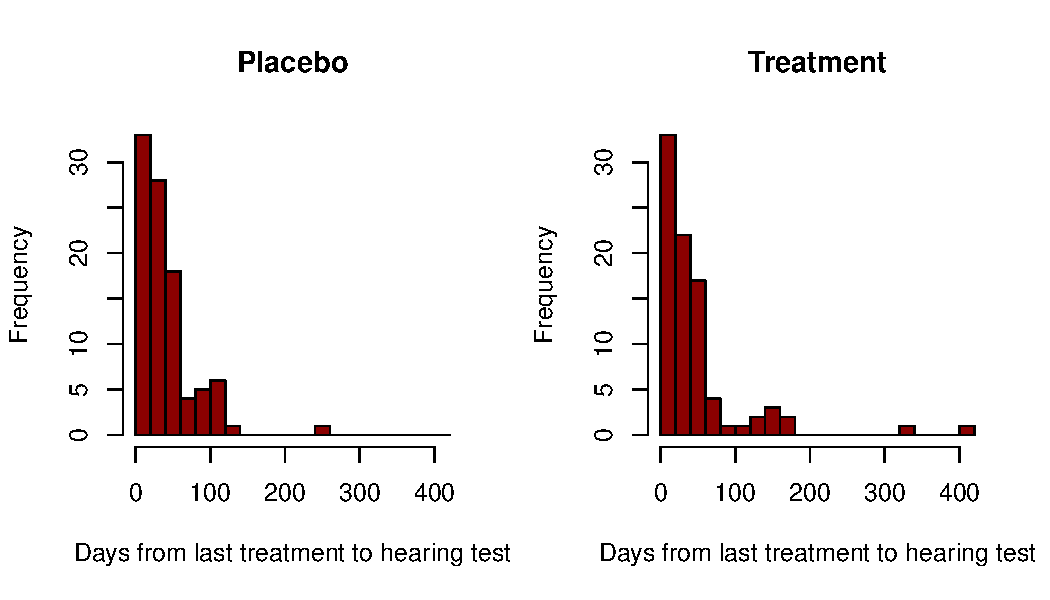
\includegraphics[width=.8\textwidth]{./rcode/plots/days_since_trt_stop}
\caption{Histogram of the number of days between treatment was stopped and the last hearing test was taken stratified by treatment.}
\label{fig:days_since_last_trt}
\end{figure}


\section{Fitted Models Supplementary Materials}
\subsection{Model I}
\label{sec:model_i_app}

\captionsetup{width=.9\textwidth}
\begin{figure}[H]
\centering
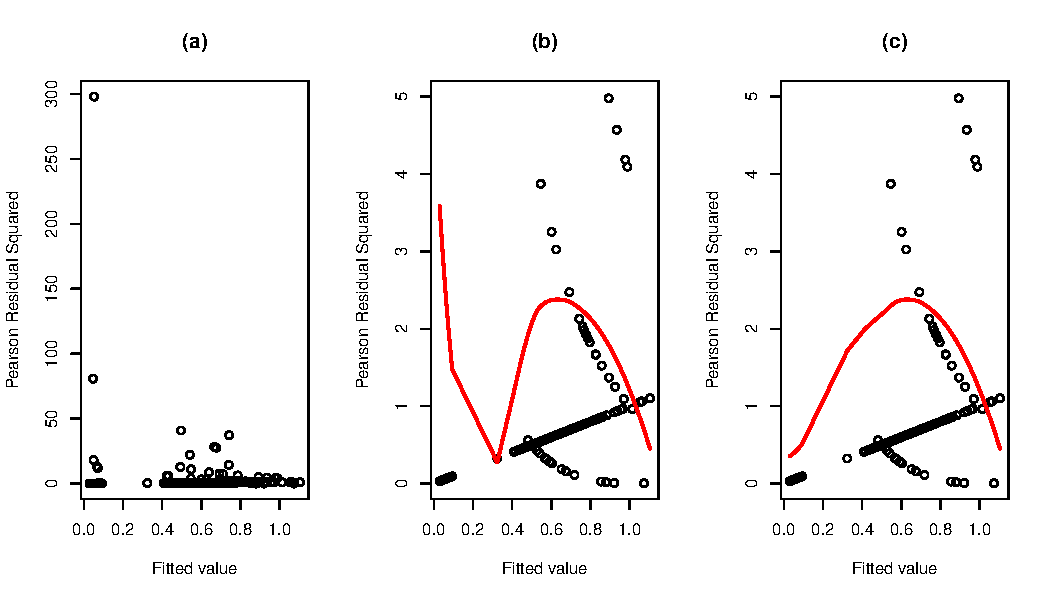
\includegraphics[width=.9\textwidth]{./rcode/plots/model_i_pearson}
\caption{Squared Pearson residuals against fitted values for model I. The red line indicates a Loess smoother. Plot (a) shows just the residuals. Plot (b) shows a Loess smoother and limits the y range. It can be seen that the smoothed line is not constant at 1. Plot (c) shows the Loess smoother when the two highest residuals are removed.}
\label{fig:model_i_pearson}
\end{figure}
\begin{figure}[H]
\centering
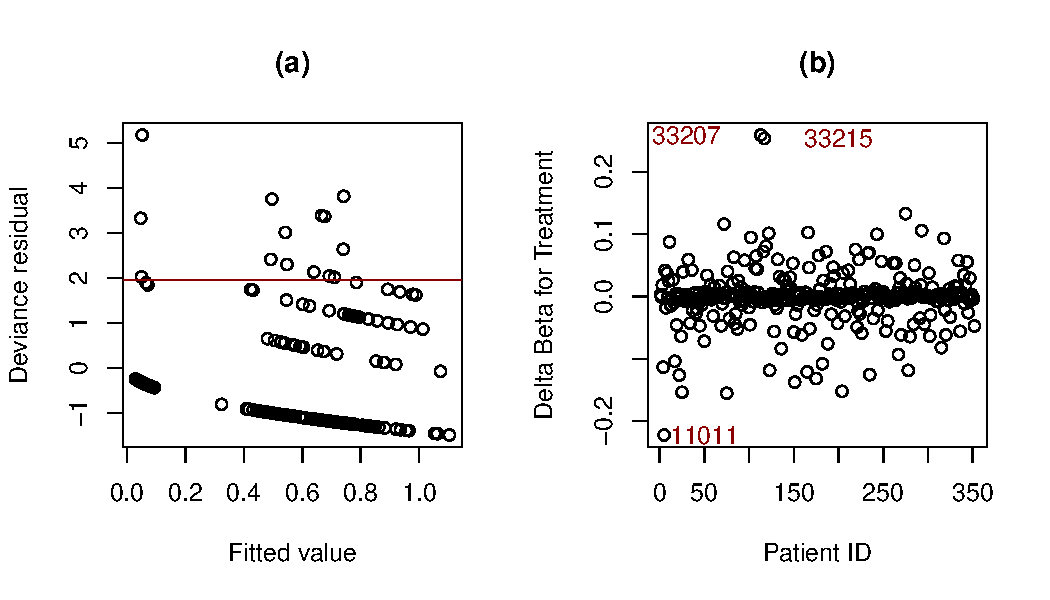
\includegraphics[width=.9\textwidth]{./rcode/plots/model_i_diagnostics}
\caption{Plot (a) shows the deviance residuals from model I. The 95\% probability interval of a standard normal distribution is indicated by the red line. Plot (b) shows delta beta values across patient IDs. Note that the patient IDs on the x-axis do not correspond to the actual in-study patient IDs. The numbers in red indicate the in-study IDs of three flagged values.}
\label{fig:model_i_diagnostics}
\end{figure}

\begin{table}[H]
\centering
\caption{Model estimates for model excluding gender}
\begin{tabular}{rll}
  \hline
 & Incidence Rate Ratio (95\% CI) & p-value \\ 
  \hline
Intercept & 1.625 (0.262, 10.078) & 0.602 \\ 
  Treatment & 0.086 (0.032, 0.23) & $<$0.001 \\ 
  Aspirin & 1.486 (0.921, 2.397) & 0.105 \\ 
  Age (yrs) & 0.983 (0.954, 1.013) & 0.262 \\ 
  African American & 0.649 (0.105, 4.003) & 0.642 \\ 
   \hline
\end{tabular}
\end{table}

\begin{table}[H]
\centering
\caption{Model estimates for model excluding African-American ethnicity}
\begin{tabular}{rll}
  \hline
 & Incidence Rate Ratio (95\% CI) & p-value \\ 
  \hline
Intercept & 1.623 (0.26, 10.125) & 0.604 \\ 
  Treatment & 0.087 (0.032, 0.232) & $<$0.001 \\ 
  Aspirin & 1.441 (0.891, 2.331) & 0.136 \\ 
  Age (yrs) & 0.982 (0.952, 1.012) & 0.232 \\ 
  Male & 1.103 (0.588, 2.069) & 0.761 \\ 
   \hline
\end{tabular}
\end{table}


\subsection{Model II}
\label{sec:model_ii_app}

\captionsetup{width=.9\textwidth}
\begin{figure}[H]
\centering
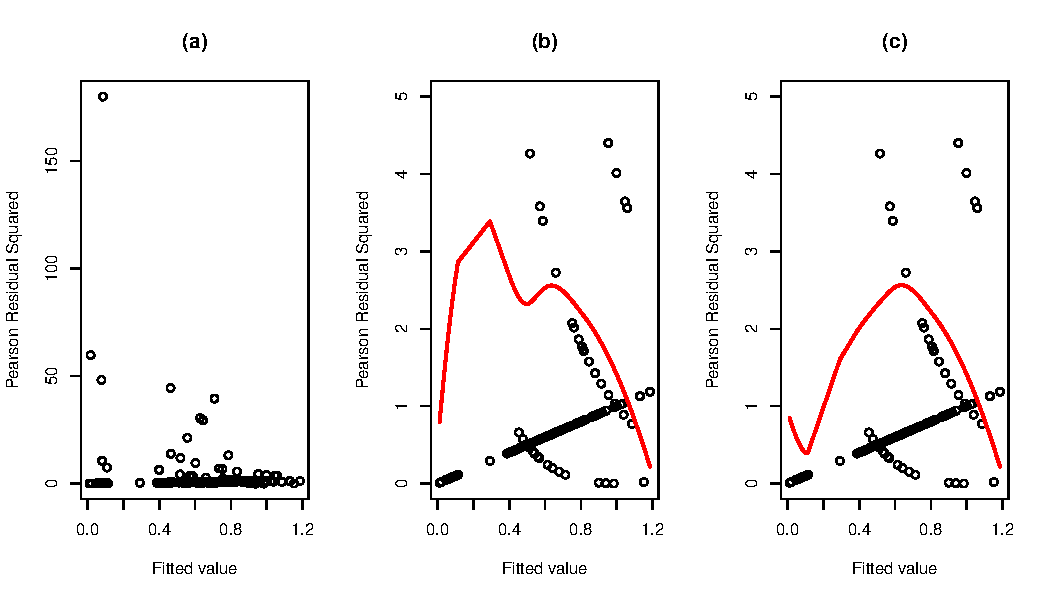
\includegraphics[width=.9\textwidth]{./rcode/plots/model_ii_pearson}
\caption{Squared Pearson residuals against fitted values for model II. The red line indicates a Loess smoother. Plot (a) shows just the residuals. Plot (b) shows a Loess smoother and limits the y range. As before it the line is not constant at 1 indicating overdispersion. The structure is similar as for model I (figure~\ref{fig:model_i_pearson}) Plot (c) shows the Loess smoother when the two highest residuals are removed.}
\label{fig:model_ii_pearson}
\end{figure}
\begin{figure}[H]
\centering
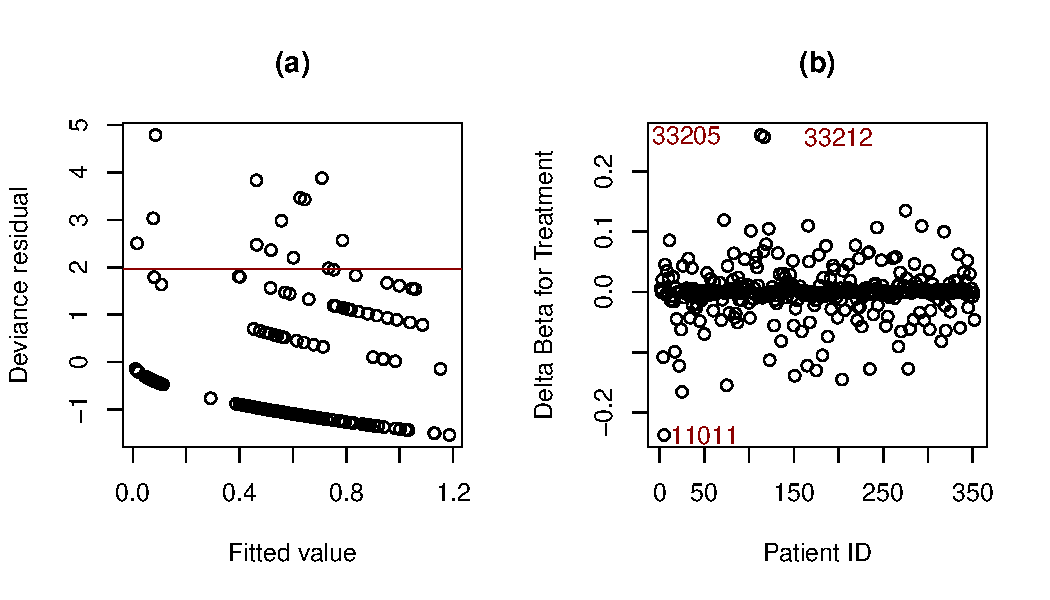
\includegraphics[width=.9\textwidth]{./rcode/plots/model_ii_diagnostics}
\caption{Plot (a) shows the deviance residuals from model II. The 95\% probability interval of a standard normal distribution is indicated by the red line. Plot (b) shows delta beta values across patient IDs for model II. Note that the patient IDs on the x-axis do not correspond to the actual in-study patient IDs. The numbers in red indicate the in-study IDs of three flagged values.}
\label{fig:model_ii_diagnostics}
\end{figure}

\subsection{Model III}
\label{sec:model_ii_app}

\captionsetup{width=.9\textwidth}
\begin{figure}[H]
\centering
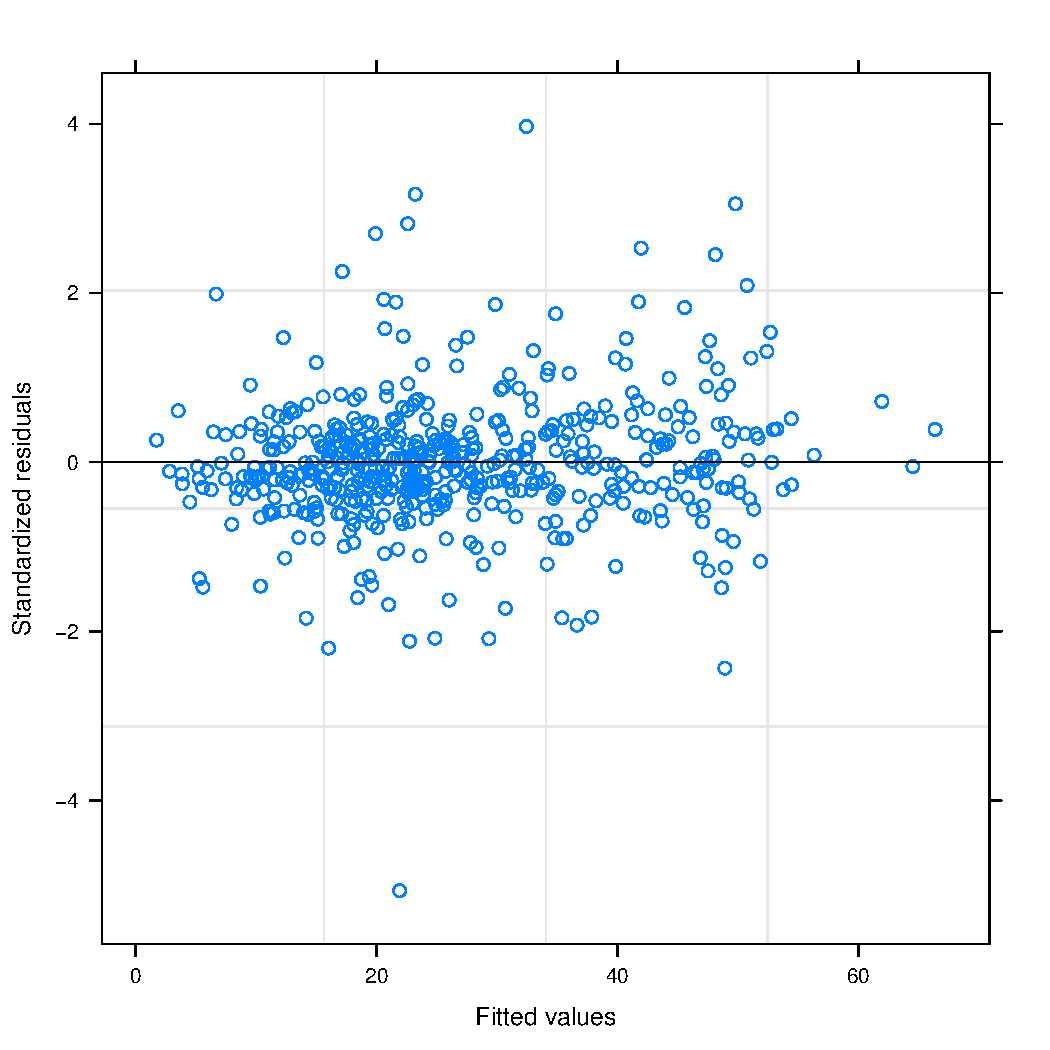
\includegraphics[width=.5\textwidth]{./rcode/plots/model_iii_resid}
\caption{Standardized residuals against fitted values for model III. There is no clear trend that indicates a mean function misspecification.}
\label{fig:model_ii_pearson}
\end{figure}
\begin{figure}[H]
\centering
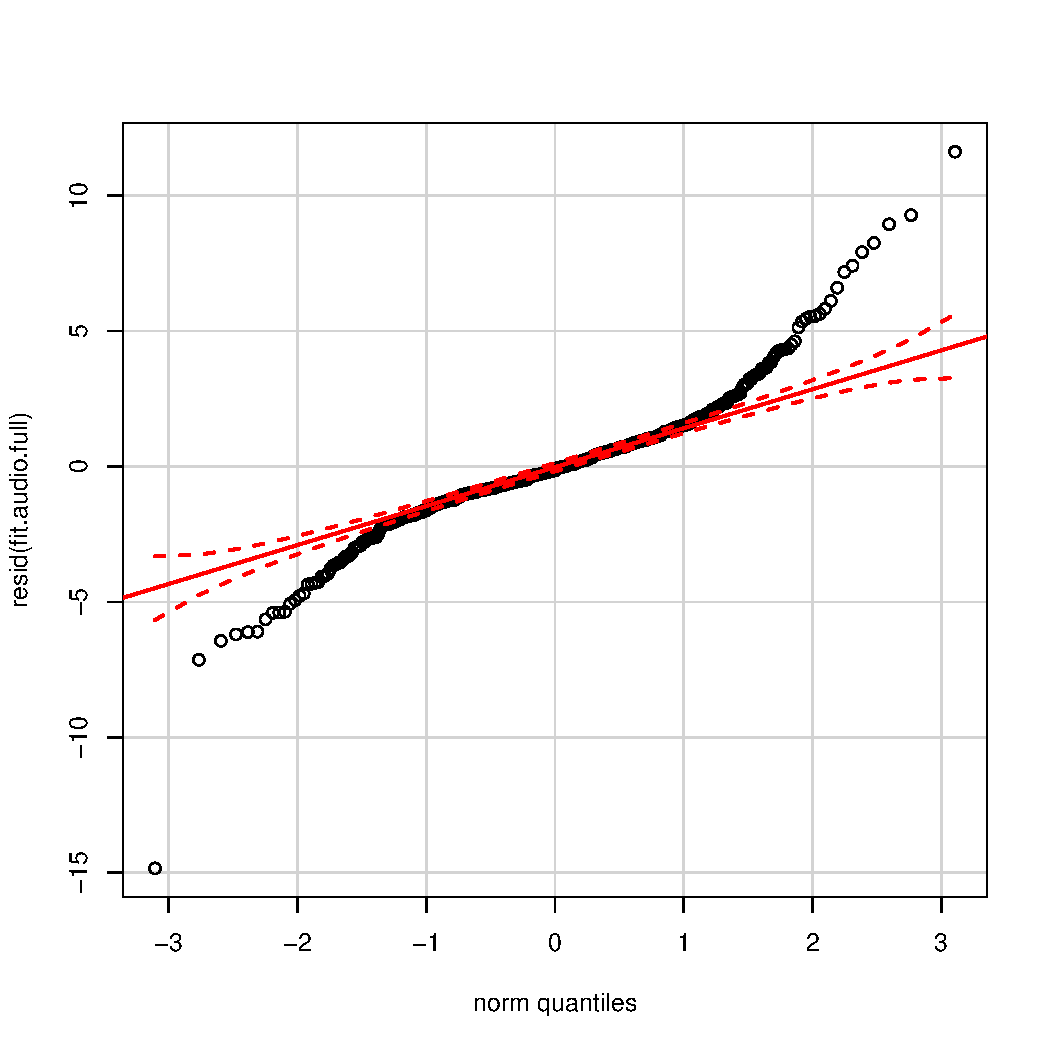
\includegraphics[width=.5\textwidth]{./rcode/plots/model_iii_qq}
\caption{Normal QQ-plot for the residuals obtained from model III. The plot indicates that the tails of the residual distribtution are thicker than for the normal distribution. This could impact the validity of the inference we draw on the mean model coefficients.}
\label{fig:model_ii_diagnostics}
\end{figure}


\end{document}